\usetikzlibrary{decorations.markings}
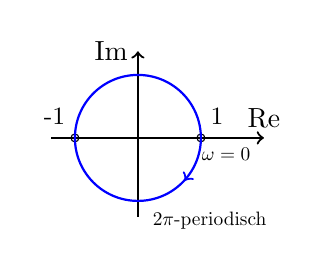
\begin{tikzpicture}
\useasboundingbox (-1.4,-1.4) rectangle (1.9,1.4);
\draw[->, thick] (-1.1,0) -- (1.6,0) node[above] {Re};
\draw[->, thick] (0,-1) -- (0,1.1) node[left] {Im};

\draw (0.8,0.05) arc(90:450:0.05) node[above right] {\small{1}};
\draw (-0.8,0.05) arc(90:450:0.05) node[above left] {\small{-1}};

\draw[blue, thick,
	decoration={
		markings,
		mark= at position 0.9 with {\arrow{<}}
	},
	postaction={decorate}
] (0.8,0) arc (0:360:0.8);

\scalebox{0.7}{
  \node at (1.3,-1.5) {$2\pi$-periodisch};
  \node at (1.6, -0.3) {$\omega = 0$};
}
%\draw (current bounding box.south west) rectangle (current bounding box.north east);
\end{tikzpicture}